\documentclass[conference]{IEEEtran}

\usepackage{cite}
\usepackage{graphicx}
\usepackage{booktabs}
\usepackage{amsmath}
\usepackage{amssymb}
\usepackage{xcolor}
\usepackage{url}
\usepackage[section]{placeins}

\newcommand{\model}{TCN-WGAN-GP with TAD Scoring}
\newcommand{\tad}{TAD Score}

\begin{document}

\title{Toward Low-Noise Window-Level Network Intrusion Detection with TCN-WGAN-GP and TAD Scoring}

\author{
\IEEEauthorblockN{Jie Li}
\IEEEauthorblockA{
School of Software, Beihang University, Beijing, China\\
Email: zb2557106@buaa.edu.cn
}
}

\maketitle

\begin{abstract}
Window-level intrusion detection is attractive for deployment because it can incorporate short-range temporal context and support explicit alarm calibration, but practical benefit depends on whether false positives remain controllable under realistic thresholds. This paper presents \model{}, a calibrated window-level anomaly detector that combines a Temporal Convolutional Network backbone, Wasserstein training with gradient penalty, and a simple Temporal Attention-Deviation (\tad{}) scoring rule. The detector is trained on benign windows from the training split and calibrated only on benign windows, while attack labels are reserved for evaluation. We evaluate the method on CICIDS2017, SWaT, UNSW-NB15, and TON\_IoT against classical and modern anomaly-detection baselines. The strongest results are obtained on CICIDS2017 and SWaT, where the detector achieves favorable low-FPR operating points under chronological or formal anomaly-detection protocols. On UNSW-NB15, the method remains competitive but exposes the difficulty of threshold transfer under distribution shift; TON\_IoT is treated as an out-of-domain limitation case. We further provide a multi-view alarm-audit analysis based on attention, Integrated Gradients, and SHAP, while explicitly avoiding the assumption that attention alone constitutes a faithful explanation.
\end{abstract}

\begin{IEEEkeywords}
network intrusion detection, low false positives, temporal convolutional network, generative adversarial network, explainable AI, anomaly detection
\end{IEEEkeywords}

\section{Introduction}
Network intrusion detection systems must identify malicious behavior from high-volume, evolving traffic while keeping false alarms low enough for deployment. A useful detector for security operations should reason over short temporal contexts, support online scoring, and provide evidence that helps analysts understand why a window of traffic was flagged.

Many machine-learning intrusion detection pipelines operate at the flow level: each flow is treated as an independent sample, and the model predicts whether that flow is benign or malicious. This formulation is simple and useful, but it can miss temporal patterns across neighboring flows and can blur runtime claims, because a strong flow-level classifier is not automatically a stable streaming detector. For a communications and network security setting, the unit of analysis should therefore match the unit of response: an alarm should summarize a recent traffic segment rather than a single isolated record.

The false-alarm constraint is especially important in operational security monitoring. A detector with high recall but excessive benign false positives may overwhelm analysts and reduce trust in alarms. For this reason, we evaluate not only ranking metrics such as AUC and average precision, but also calibrated operating points under explicit false-positive-rate budgets.

This paper studies a window-level alternative. We convert consecutive network flows into fixed-length windows and train a TCN-GAN model to capture benign temporal structure. To improve stability and make the scoring rule more deployment-oriented, we upgrade the basic TCN-GAN with WGAN-GP, short for Wasserstein Generative Adversarial Network with Gradient Penalty, and an attention-aware scoring mechanism. We call the resulting framework \model{}. At inference time, the detector computes a Temporal Attention-Deviation (\tad{}) anomaly score that combines attention-aware critic evidence with feature-space deviation from benign reference windows.

Our target claim is deliberately narrow and testable: after fixing the window size, stride, and score-fusion ratio, \model{} should provide a competitive low-noise operating point under a window-level protocol and offer useful post-hoc evidence for alarmed windows. We do not claim global hyperparameter optimality or universal dominance across all traffic domains.

This paper makes the following contributions:
\begin{itemize}
  \item We present \model{}, a calibrated window-level TCN-WGAN-GP detector with a simple \tad{} scoring rule that combines attention-aware critic evidence and benign-reference feature deviation.
  \item We define an operational evaluation protocol based on chronological or formal anomaly-detection splits, benign-only training and calibration, explicit target-FPR operating points, and fixed window-level comparison settings.
  \item We provide an empirical study of low-FPR behavior, cross-dataset transfer, ablation, and multi-view alarm-audit analysis, highlighting both the settings in which the detector is effective and the boundary cases in which it is not.
\end{itemize}

\section{Background and Motivation}
\subsection{Operational Monitoring Goal}
We consider a network monitoring setting in which a defender observes flow-level telemetry from an enterprise, cloud, or industrial network and must raise timely alarms for suspicious traffic segments. The proposed detector is trained on benign windows from the training split, which reflects the common deployment assumption that representative attack variants may not be available during training. Attack labels are used for evaluation, model-selection analysis, and comparison with baselines, but they are not used to optimize the adversarial detector or to calibrate its deployment threshold.

The security goal is not to assign a perfect semantic attack label to every flow. Instead, the goal is to produce a low-noise alarm stream that prioritizes windows likely to contain malicious behavior. This framing makes three requirements central: the alarm unit should preserve short-term traffic context, the threshold should be calibrated under an explicit false-positive budget, and the final alarm should be inspectable enough for an analyst to decide whether escalation is warranted.

\subsection{Window-Level Detection}
Let a network trace be represented as an ordered sequence of flow feature vectors. A flow-level detector maps each vector to a label independently. In contrast, a window-level detector maps a sequence window to a score:
\begin{equation}
  X_i = [x_i, x_{i+1}, \ldots, x_{i+W-1}], \quad s_i = f(X_i),
\end{equation}
where $W$ is the window size and consecutive windows are separated by stride $r$. This formulation is better aligned with real-time monitoring because the detector can emit an alarm whenever the score of the current window exceeds a calibrated threshold.

The choice of $W$ and $r$ controls a trade-off. Larger windows contain more temporal context but increase latency and memory use; smaller strides improve temporal resolution but create more windows and higher compute cost. Our experiments therefore report both detection quality and throughput.

\subsection{Temporal Convolutional Networks and GANs}
Temporal convolutional networks use causal or dilated one-dimensional convolutions to capture sequence patterns efficiently \cite{bai2018tcn}. GANs train a generator and discriminator in an adversarial objective \cite{goodfellow2014gan}; for anomaly detection, the discriminator can learn a boundary around normal data. Because vanilla GAN training may be unstable, Wasserstein GAN (WGAN) objectives and WGAN-GP, namely Wasserstein Generative Adversarial Network with Gradient Penalty, are often used to improve critic training \cite{arjovsky2017wgan,gulrajani2017wgangp}. The Wasserstein objective replaces binary real/fake classification with a critic score that approximates the distance between the real and generated distributions, while the gradient penalty regularizes the critic to satisfy the Lipschitz constraint required by the Wasserstein formulation.

\section{Related Work}
\subsection{Network Intrusion and Anomaly Detection}
Classical intrusion detection pipelines often use flow-level features and supervised or one-class models. Earlier benchmarks such as KDD Cup 1999 and NSL-KDD helped standardize IDS evaluation, but their traffic distributions and attack patterns are widely considered limited for modern network settings \cite{tavallaee2009nslkdd}. Later datasets such as UNSW-NB15 and CICIDS2017 introduced more diverse flow features and attack scenarios \cite{moustafa2015unsw,sharafaldin2018cicids}. CICIDS2017 remains a common benchmark because it contains benign traffic and several attack families collected across multiple days.

Traditional machine-learning detectors include tree ensembles, support-vector methods, nearest-neighbor methods, and one-class anomaly detectors. Isolation Forest isolates anomalous points using random partitioning \cite{liu2008iforest}, while One-Class SVM estimates a boundary around normal samples \cite{scholkopf2001ocsvm}. These methods are useful baselines because they are simple and strong on tabular flow features. However, independent flow classification can miss temporal evidence that emerges across adjacent flows, and threshold calibration can strongly affect recall and false positives.

Unsupervised and online anomaly detection methods reduce dependence on attack labels. Kitsune, for example, uses an ensemble of autoencoders for online network intrusion detection and emphasizes deployability on resource-constrained devices \cite{mirsky2018kitsune}. Recent work has also explored Transformer-based NIDS frameworks and cloud-security intrusion detectors, showing that attention architectures are increasingly relevant for flow-based security analytics \cite{manocchio2024flowtransformer,long2024transformercloud,xi2024multiscale}. A particularly related direction combines GANs, TCNs, and self-attention for unsupervised intrusion detection \cite{araujo2023unsupervised}; recent IP-flow GAN work also evaluates TCN, LSTM, and CNN variants with SHAP-based analysis on CIC-style traffic datasets \cite{ruffo2025ganipflow}. Our work shares the goal of online anomaly detection, but differs in its explicit low-FPR calibration protocol, WGAN-GP ablation, \tad{}-based anomaly scoring, and multi-view XAI case study.

\subsection{Deep Sequence Models for Anomaly Detection}
Deep anomaly detection has used recurrent, convolutional, forecasting-based, Transformer-based, and autoencoder-based models to capture temporal or reconstruction patterns. Recurrent models have been used for time-series anomaly detection and log anomaly detection, where the model learns expected sequential behavior and flags deviations \cite{malhotra2016lstm,du2017deeplog}. Autoencoder variants reconstruct normal inputs and treat high reconstruction error as evidence of abnormality \cite{sakurada2014autoencoder,an2015vae}. DeepSVDD trains a deep representation using a one-class objective \cite{ruff2018deep}, while TranAD uses Transformer encoders for multivariate time-series anomaly detection \cite{tuli2022tranad}. Recent general time-series models such as Anomaly Transformer and TimesNet further show the importance of attention, association, and temporal variation modeling for unsupervised anomaly detection \cite{xu2022anomalytransformer,wu2023timesnet}. A recent review of time-series analysis for cyber security further highlights intrusion detection as a key application area and emphasizes challenges such as heterogeneous feature types, sparsity, and temporal aggregation \cite{landauer2025timeseriessecurity}. Industrial IoT anomaly-detection work has also moved toward dynamic and adaptive sequence models for multivariate telemetry \cite{kong2025dadn}. These approaches are natural for sequence data, but recurrent or Transformer evaluation can be slower, and reconstruction quality does not always align with detection quality.

Temporal convolutional networks offer a practical alternative because dilated convolutions can capture long-range sequence patterns with efficient parallel computation \cite{bai2018tcn}. Compared with recurrent models, TCNs are easier to batch across windows and can provide predictable inference latency. Our method uses TCN blocks inside an adversarial detector and reports window-level throughput to keep the real-time monitoring claim grounded.

\subsection{GAN-Based Detection and Training Stability}
GAN-based anomaly detection uses adversarial training to learn a normal-data manifold, a discriminator boundary, or an embedding where abnormal samples are easier to separate. AnoGAN showed that GANs can support anomaly detection by comparing samples with generated normal patterns \cite{schlegl2017anogan}, while later variants such as f-AnoGAN improved inference efficiency \cite{schlegl2019fanogan}. GANomaly introduced an encoder-decoder-encoder adversarial detector that has become a common deep anomaly baseline \cite{akcay2018ganomaly}. However, vanilla GAN objectives can be unstable, especially under imbalanced or limited-data settings. WGAN and WGAN-GP improve training by replacing the discriminator classification objective with a Wasserstein critic and gradient penalty \cite{arjovsky2017wgan,gulrajani2017wgangp}. Our ablation explicitly evaluates whether WGAN-GP improves a TCN-based adversarial detector when the window size, stride, and score fusion are held fixed.

\subsection{Explainability and Attention}
XAI is increasingly important for security systems because analysts need to understand why an alarm was raised, not only whether it was raised. Feature-attribution methods such as saliency maps, Integrated Gradients, LIME, and SHAP provide post-hoc explanations of model predictions \cite{simonyan2014saliency,sundararajan2017axiomatic,ribeiro2016lime,lundberg2017shap}. Recent IDS studies have increasingly combined attention models with SHAP, LIME, drift awareness, and cross-dataset evaluation to improve analyst trust \cite{rahman2025explaining,sehgal2026adaptive}. Attention weights can also expose where a model aggregates evidence, but attention should not automatically be treated as a faithful explanation of the final prediction \cite{jain2019attention}. For this reason, we report both attention weights and attribution methods: attention describes temporal aggregation inside the discriminator, while Integrated Gradients and SHAP estimate which time steps and traffic features contribute to the final anomaly score.

\section{Method}
\subsection{Data Representation}
Given numeric flow features, we clean and scale each feature, preserve the temporal order within each file split, and construct sliding windows of length $W$. A window is labeled anomalous if at least a fraction $\rho$ of its contained flows are labeled as attacks. In the main experiments, $\rho=0.15$. This produces the window-level evaluation target used throughout the paper.

This representation is intentionally different from a flow-level classifier. The input to the detector is not a single flow vector, but a short ordered traffic segment. The window label is used only for evaluation and for supervised baselines; the adversarial detector itself is trained only on benign windows. As traffic arrives, the system advances by stride $r$, forms the newest window, computes an anomaly score, and compares it with a calibrated threshold.

\begin{figure}[!t]
  \centering
  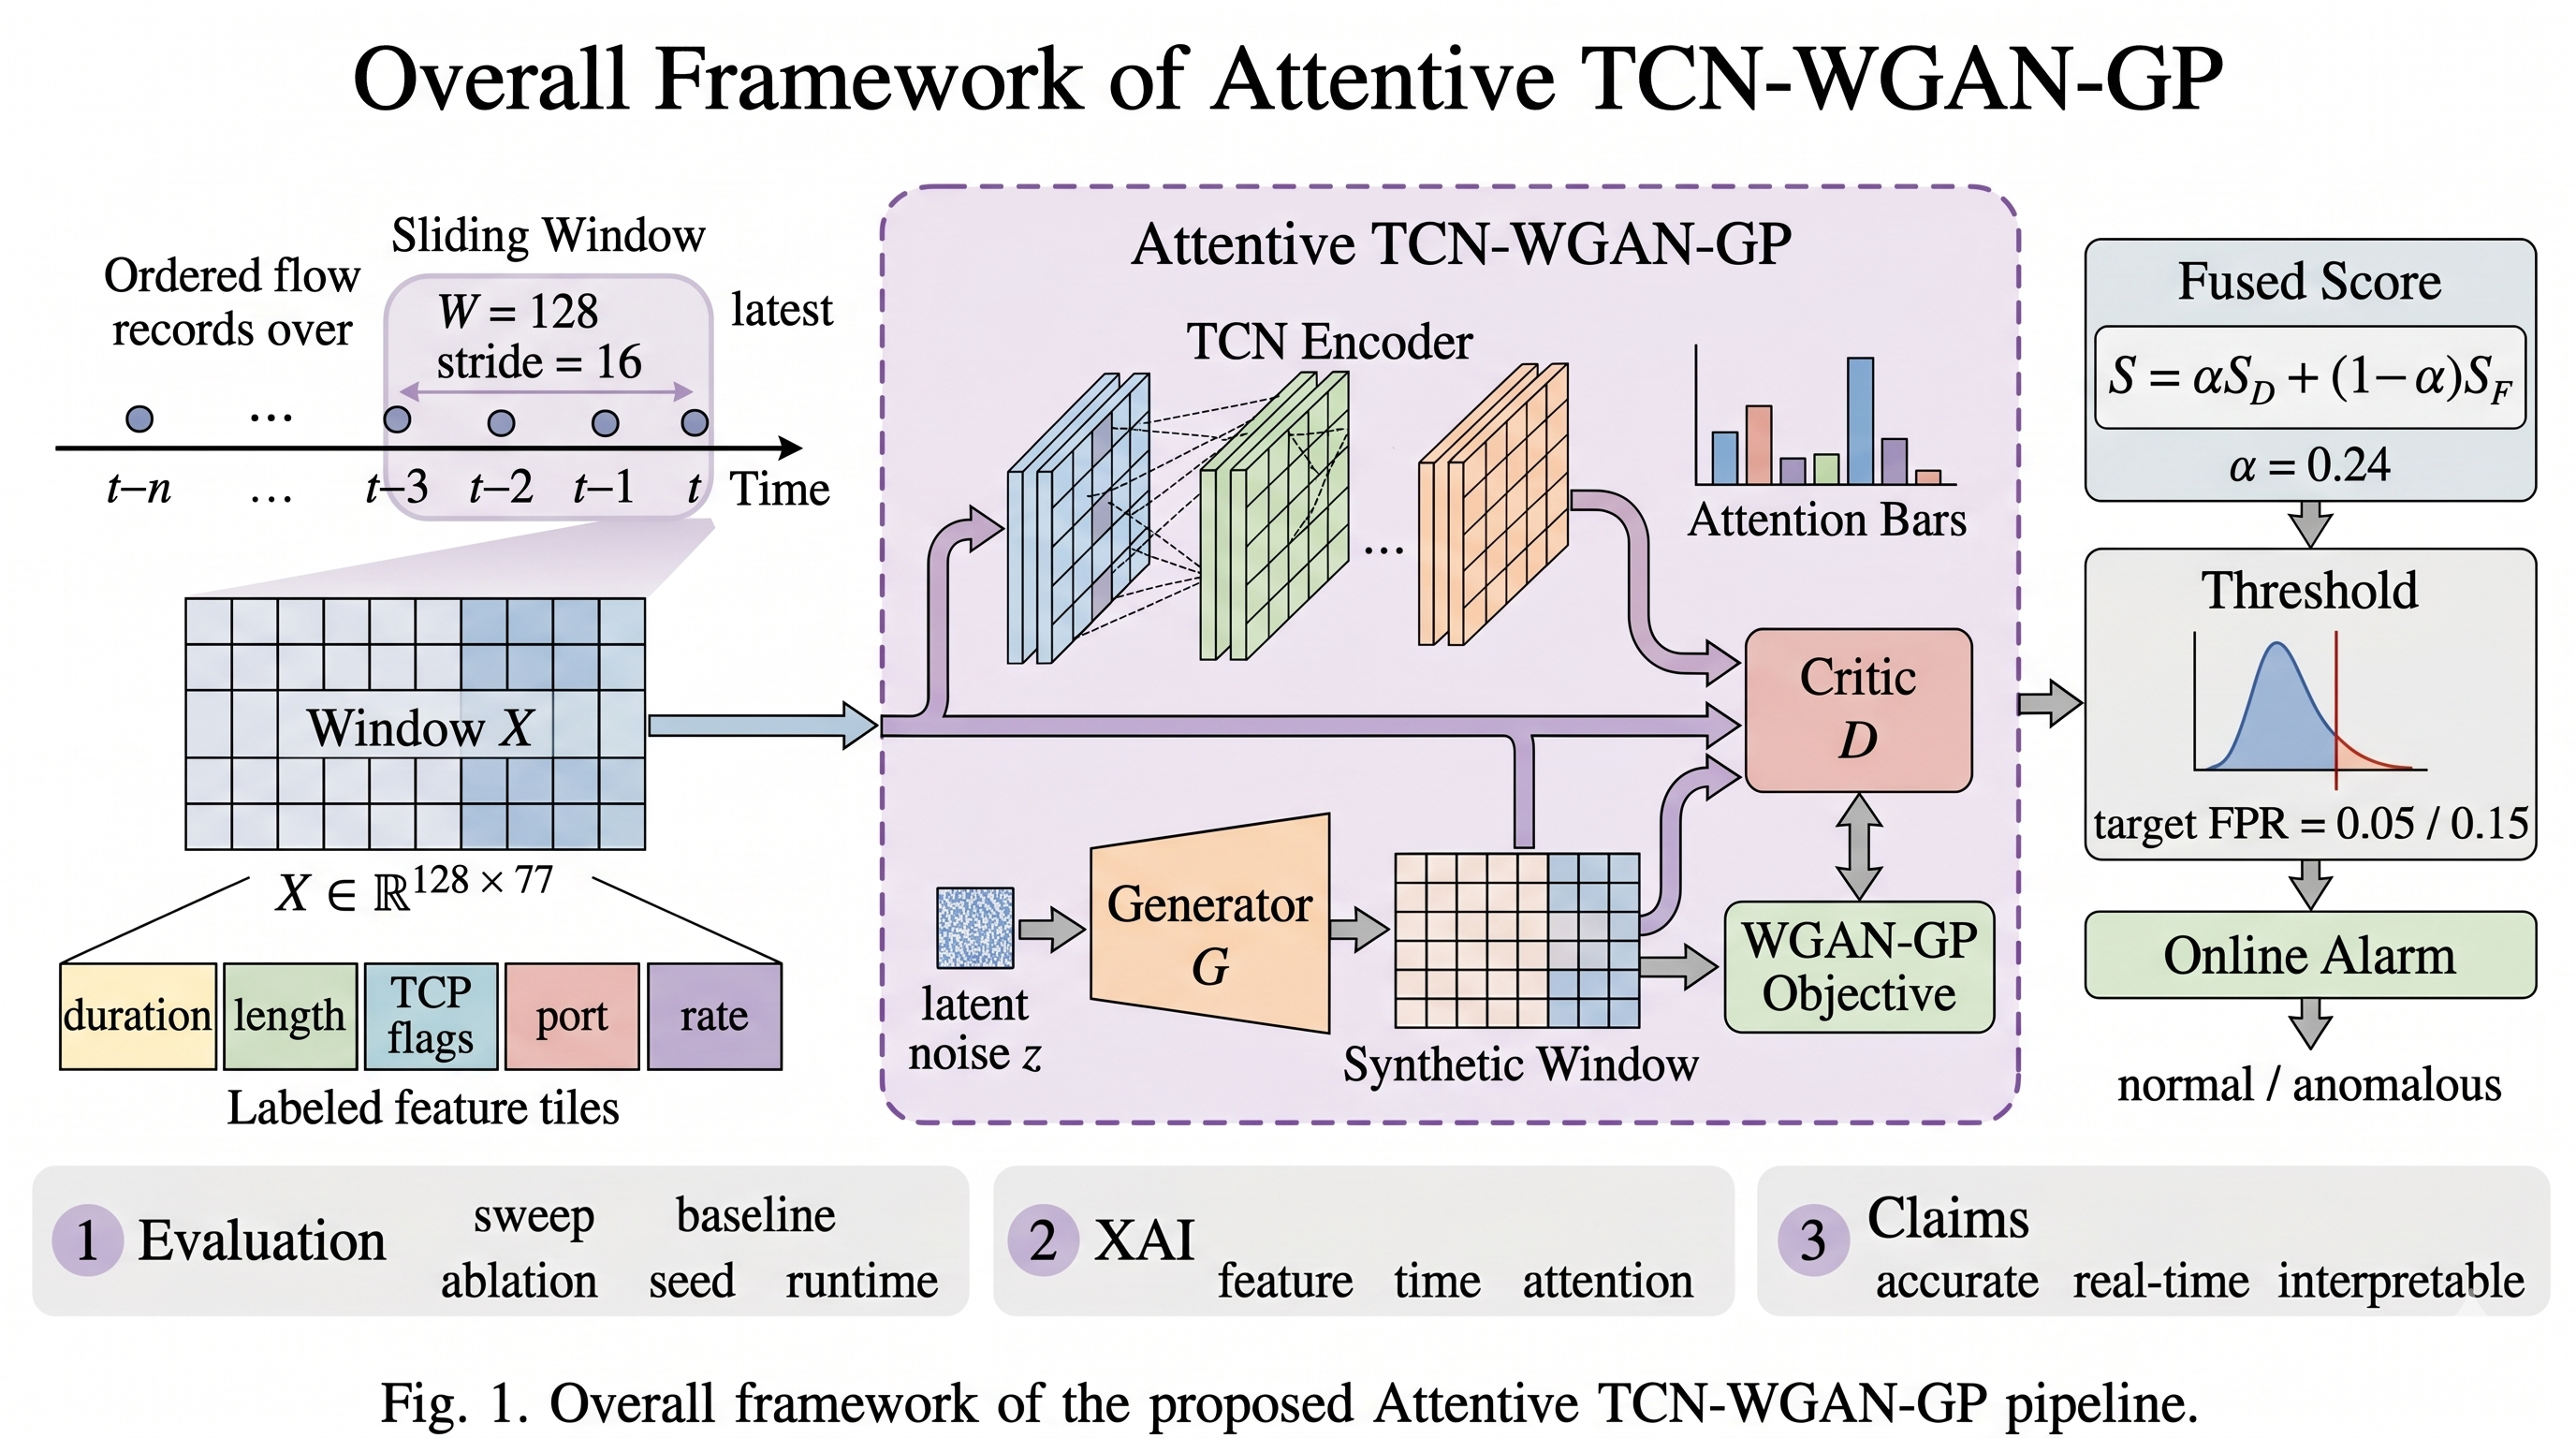
\includegraphics[width=\linewidth,height=0.28\textheight,keepaspectratio]{figures/framework_overview.png}
  \caption{End-to-end workflow of the proposed window-level intrusion detection framework. Flow records are cleaned, scaled, converted into sliding windows, scored by the trained detector, calibrated under a benign false-positive budget, and audited with post-hoc XAI evidence.}
  \label{fig:framework-overview}
\end{figure}

\subsection{Modeling the Detector Upgrade}
We name the proposed framework \model{} to emphasize that the main detection output is the score, not merely the backbone choice. ``TCN'' refers to the Temporal Convolutional Network backbone used for window modeling, ``WGAN-GP'' refers to Wasserstein Generative Adversarial Network with Gradient Penalty, and ``TAD'' refers to Temporal Attention-Deviation scoring. In our usage, ``attention-deviation'' does not mean a third separately trained network branch; it means that the final score combines an attention-aware critic response with explicit deviation from benign hidden representations.

The proposed model can be viewed as an upgrade from a basic TCN-GAN detector to a TCN-WGAN-GP detector with \tad{} scoring. Let $X\in\mathbb{R}^{W\times d}$ denote a traffic window with $W$ time steps and $d$ flow features. The generator $G_\theta$ maps latent noise $z\sim p(z)$ to a synthetic benign-like window,
\begin{equation}
  \tilde{X}=G_\theta(z), \quad \tilde{X}\in\mathbb{R}^{W\times d},
\end{equation}
and the discriminator or critic $D_\phi$ maps a real or generated window to a scalar evidence score. The basic TCN-GAN version uses TCN encoders in both $G_\theta$ and $D_\phi$ and trains them with a standard adversarial real/fake objective:
\begin{align}
  \mathcal{L}^{\mathrm{vanilla}}_D =
  &-\mathbb{E}_{X\sim P_r}[\log \sigma(D_\phi(X))] \nonumber\\
  &-\mathbb{E}_{z\sim p(z)}[\log(1-\sigma(D_\phi(G_\theta(z))))],
\end{align}
\begin{equation}
  \mathcal{L}^{\mathrm{vanilla}}_G =
  -\mathbb{E}_{z\sim p(z)}[\log \sigma(D_\phi(G_\theta(z)))].
\end{equation}
This baseline gives a temporal adversarial detector, but it has two weaknesses: the discriminator aggregates all time steps uniformly, and the vanilla GAN objective can be unstable. We therefore model the final detector as three explicit modifications:
\begin{equation}
\begin{aligned}
  M_0 &= \mathrm{TCN\text{-}GAN},\\
  M_1 &= M_0 + \mathrm{attention\ pooling},\\
  M_2 &= M_1 + \mathrm{WGAN\text{-}GP},\\
  S(X) &= \mathrm{\tad{} scoring}(M_2, X).
\end{aligned}
\end{equation}
The first modification changes temporal aggregation, the second changes the adversarial training objective, and the third changes the inference-time anomaly score. This formulation makes the model upgrade measurable in ablation.

\subsection{\model{} Architecture}
The final implementation uses two TCN blocks with hidden channels $[128,128]$, kernel size $3$, dilations $\{1,2\}$, dropout $0.2$, latent dimension $64$, and a $1\times1$ output projection. The generator receives a latent vector $z$ and maps it through a linear layer followed by the TCN stack and a $1 \times 1$ convolution to produce a synthetic window. The discriminator maps an input window through the same-depth TCN stack to obtain temporal hidden features. A time-wise classifier produces logits for each time step. With mean pooling, the discriminator averages these logits. With attention pooling, the discriminator applies a learned linear projection over time steps and aggregates the logits by weighted sum:
\begin{equation}
  D(X) = \sum_{t=1}^{W} a_t \ell_t,\quad
  q_t = w_a^\top h_t + b_a,\quad
  a_t = \frac{\exp(q_t)}{\sum_{j=1}^{W}\exp(q_j)}.
\end{equation}
Here $h_t$ is the discriminator hidden state, $\ell_t$ is the discriminator logit at time $t$, and $a_t$ is the normalized attention weight. In code, the projection is implemented as a lightweight $1\times1$ convolution followed by softmax over time.

The attention module is not introduced as a stand-alone explanation method. It is a learnable pooling mechanism inside the discriminator. Mean pooling assumes that all positions in the window contribute equally to the discriminator score, while attention pooling allows the model to emphasize positions that provide stronger evidence about whether the whole window resembles benign traffic.

\begin{figure}[!t]
  \centering
  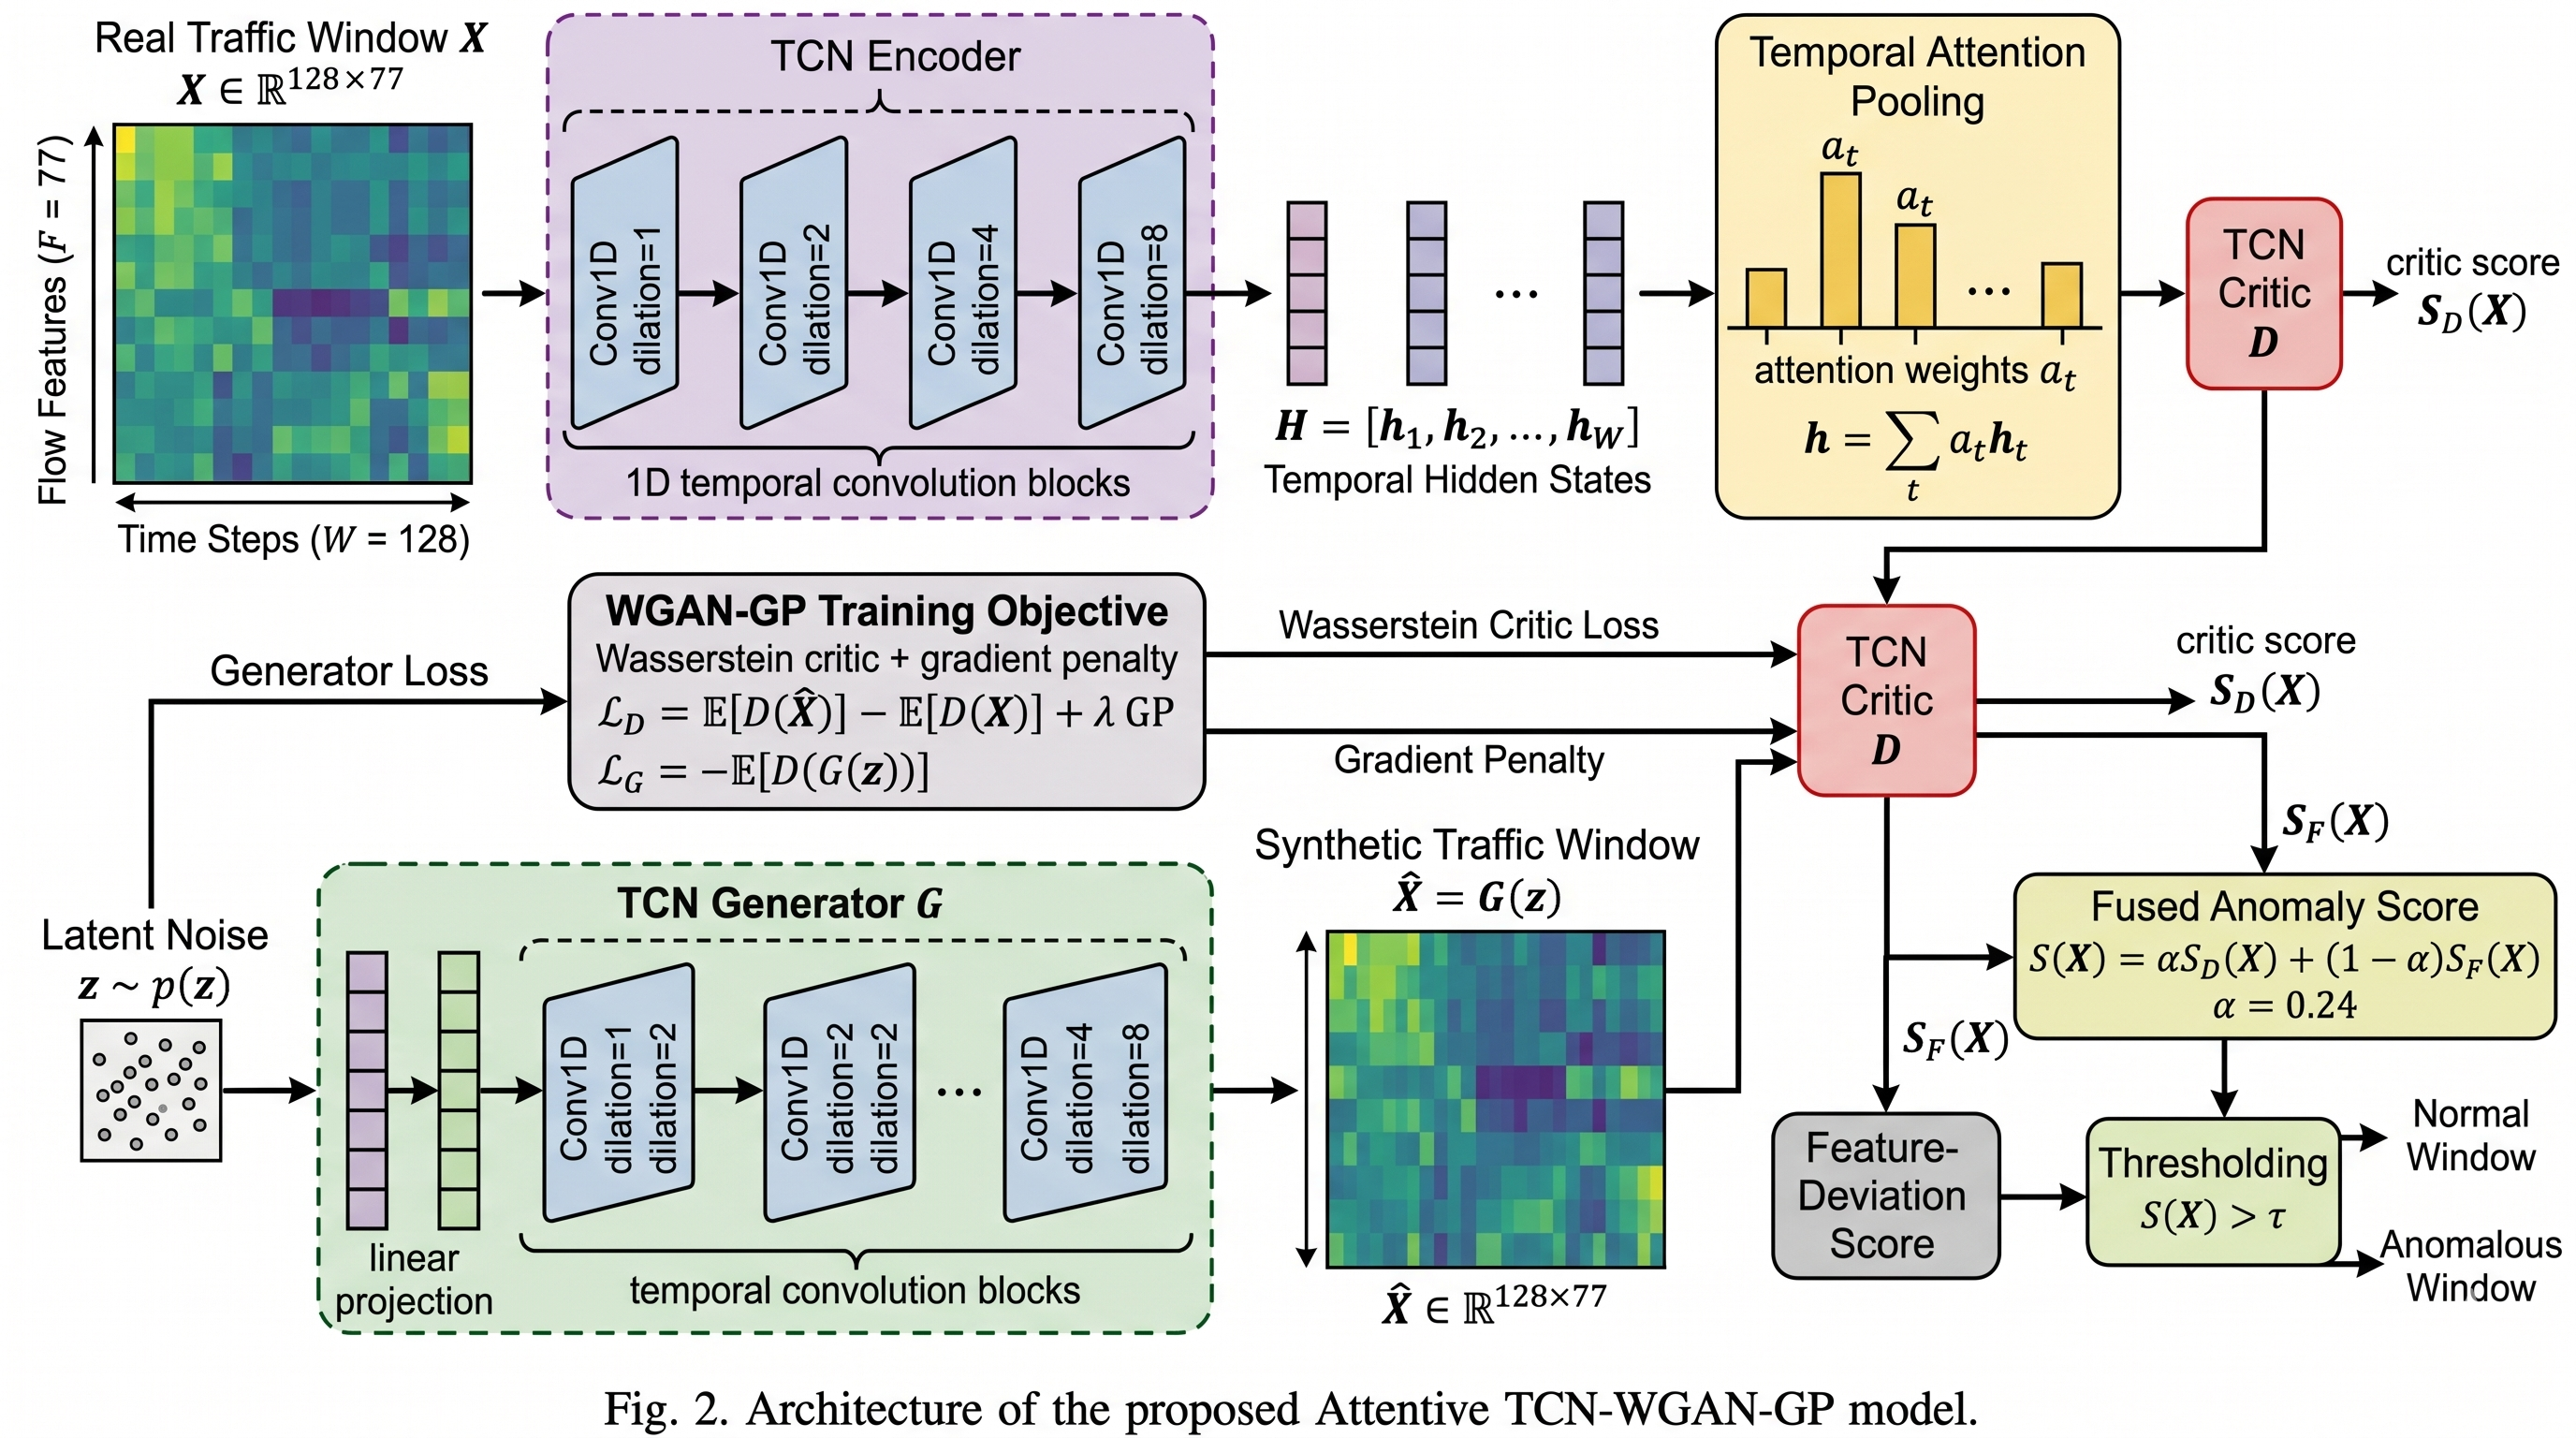
\includegraphics[width=\linewidth,height=0.34\textheight,keepaspectratio]{figures/model_architecture.png}
  \caption{Architecture of \model{}. A TCN generator synthesizes benign-like windows, while a TCN critic with attention pooling scores real and generated windows. WGAN-GP stabilizes adversarial training, and \tad{} scoring combines critic and representation-deviation evidence at inference time.}
  \label{fig:model-architecture}
\end{figure}

\subsection{WGAN-GP Training}
WGAN-GP stands for Wasserstein Generative Adversarial Network with Gradient Penalty. In this variant, the discriminator is treated as a critic rather than a probability classifier. The critic assigns larger scores to real benign windows and smaller scores to generated windows, and the gradient penalty constrains the critic to change smoothly between real and generated samples. The critic minimizes:
\begin{align}
  \mathcal{L}_D =
  &\ \mathbb{E}_{\tilde{X}\sim P_g}[D(\tilde{X})]
  - \mathbb{E}_{X\sim P_r}[D(X)] \nonumber\\
  &+ \lambda \mathbb{E}_{\hat{X}}
  [(\lVert \nabla_{\hat{X}} D(\hat{X}) \rVert_2 - 1)^2],
\end{align}
while the generator minimizes:
\begin{equation}
  \mathcal{L}_G = -\mathbb{E}_{\tilde{X}\sim P_g}[D(\tilde{X})].
\end{equation}
The main training configuration uses Adam with learning rate $3\times10^{-4}$, betas $(0.5,0.999)$, batch size $256$, 32 epochs, gradient-penalty coefficient $\lambda=10$, and five critic updates per generator update.

\subsection{Temporal Attention-Deviation Scoring}
The discriminator score captures how real the window appears to the discriminator. We also compute a feature-deviation score by embedding windows with discriminator features and measuring the distance to a benign reference distribution. Both scores are min-max normalized with benign reference statistics and fused:
\begin{equation}
  S_{\mathrm{TAD}}(X) = \alpha S_D^{\mathrm{attn}}(X) + (1-\alpha)S_F(X),
\end{equation}
where $S_D^{\mathrm{attn}}$ is the attention-aware critic unknownness score and $S_F$ is the feature-deviation score. We refer to the fused score as \tad{} because it combines temporal attention-aware evidence with deviation from benign hidden representations. The final threshold is calibrated on benign windows to target a fixed false positive rate.

This fused score is useful because the critic and the feature embedding capture related but not identical evidence. The critic score reflects the adversarial realness signal learned during GAN training, whereas the feature-deviation score compares the hidden representation of a test window against benign reference statistics. The parameter $\alpha$ controls this trade-off. The selected main configuration uses $\alpha=0.24$, which gives more weight to deviation evidence while preserving a high-precision critic signal.

\subsection{Score Stability Analysis}
The paper does not claim a formal optimality theorem for false positives, but two stability properties are relevant. First, WGAN-GP regularizes the critic toward a 1-Lipschitz mapping \cite{gulrajani2017wgangp}. If the learned critic satisfies $\|\nabla_X D(X)\|_2 \leq K_D$ in the neighborhood of benign windows, then score perturbations caused by small input drift are bounded by
\begin{equation}
  |D(X+\Delta)-D(X)| \leq K_D \|\Delta\|_2.
\end{equation}
This is useful for intrusion detection because excessively sharp critics can produce unstable tail behavior near the decision threshold.

Second, the \tad{} fusion inherits a corresponding bound. If the feature-deviation component is $K_F$-Lipschitz, then
\begin{equation}
  |S_{\mathrm{TAD}}(X+\Delta)-S_{\mathrm{TAD}}(X)|
  \leq \left(\alpha K_D + (1-\alpha)K_F\right)\|\Delta\|_2.
\end{equation}
The bound does not guarantee a specific FPR, but it shows why the fusion coefficient $\alpha$ directly controls the score sensitivity. In practice, the operating-point FPR is imposed empirically by benign-only quantile calibration rather than by claiming that the adversarial objective alone enforces a false-positive budget.

\subsection{Explainability}
For post-hoc explanation, we compute gradient-times-input and Integrated Gradients style attributions over the final anomaly score:
\begin{equation}
  A_{t,k} = \left| X_{t,k} \frac{\partial S(X)}{\partial X_{t,k}} \right|.
\end{equation}
We summarize attributions over time and over features separately, and compare benign and anomalous windows. When attention pooling is enabled, we also report the learned temporal attention weights. For a single-window case study, we additionally compute SHAP GradientExplainer attributions with a benign background set of 64 windows. These explanations are not used to train the current model; they are used to audit whether alarms are driven by plausible temporal regions and features. Attention is therefore treated as an internal evidence aggregation signal, not as a faithful explanation by itself. Our current faithfulness check is indirect: if attention consistently highlights the same regions that dominate Integrated Gradients and SHAP evidence, confidence in the alarm audit increases, whereas disagreement is interpreted as a warning that attention alone is insufficient.

\section{Experimental Setup}
\subsection{Datasets and Splits}
We use CICIDS2017 as the main benchmark \cite{sharafaldin2018cicids}. The split is chronological by file rather than random over all windows, which reduces leakage of day-specific traffic conditions. Concretely, training uses earlier-day files, while testing is performed on Friday files that are fully unseen during training. For the proposed anomaly detector, only benign windows from the training split are used for model fitting; attack labels from the training files are not used to optimize the detector or set its threshold.

To test whether the detector generalizes beyond the main benchmark, we add three cross-dataset evaluations. SWaT is used as an industrial-control validation setting \cite{goh2016swat}, where benign data are split into train, calibration, and benign-test segments, and the attack file is used as the anomalous test segment. Recent SWaT-focused work continues to use autoencoder-style detectors for ICS anomaly detection, reinforcing SWaT as an active industrial-control benchmark \cite{aslam2024improvedaeics}. UNSW-NB15 \cite{moustafa2015unsw} is used as a third authoritative IDS dataset with its official training and testing CSV files; we use numeric features and remove identifiers and categorical labels. TON\_IoT \cite{alsaedi2020toniot} is treated as a cross-domain telemetry challenge set rather than as a primary win condition, because its Linux telemetry stream differs substantially from flow and process-control traffic. Recent work also evaluates hybrid IDS models on UNSW-NB15 and TON\_IoT, reinforcing their role as useful but challenging cross-dataset benchmarks \cite{chavan2025hybrid}.

All methods are evaluated at the window level with stride $r=16$ and anomaly-ratio threshold $\rho=0.15$. The main proposed model and in-repository baselines use $W=128$. External sequence baselines that impose or conventionally use a different input length are reported with their window length explicitly shown in the result tables. A window is anomalous if at least 15\% of its contained records are labeled as attacks. This keeps the evaluation granularity visible and avoids mixing flow-level and window-level claims.

\subsection{Baselines}
The main comparison uses same-granularity window-level baselines: IsolationForest, OneClassSVM, Random Forest, MLP, LSTM-AE, and LSTM-AD. We further add modern anomaly-detection baselines, including GANomaly \cite{akcay2018ganomaly}, DeepSVDD \cite{ruff2018deep}, a compact TranAD-style Transformer reconstruction model \cite{tuli2022tranad}, Anomaly Transformer \cite{xu2022anomalytransformer}, TimesNet \cite{wu2023timesnet}, and ALoRa \cite{alora_repo}. We additionally ran Time-Series-Library family variants, DLinear \cite{zeng2023dlinear} and Autoformer \cite{wu2021autoformer}, under the same window-level protocol as supplementary external references, following the Time-Series-Library benchmark line \cite{wu2023timesnet,wang2024tssurvey}. Legacy flow-level results are not mixed into the main comparison because their sample granularity differs from the proposed window-level detector.

The baseline set covers four groups. IsolationForest and OneClassSVM represent classical unsupervised anomaly detection. Random Forest and MLP represent supervised window-level classifiers trained with window labels. LSTM-AE and LSTM-AD represent deep sequence baselines based on reconstruction or sequence modeling. GANomaly, DeepSVDD, TranAD, Anomaly Transformer, TimesNet, ALoRa, and supplementary Time-Series-Library variants (DLinear and Autoformer) represent modern deep anomaly-detection baselines. This grouping helps separate the benefit of temporal benign-pattern modeling from the effects of supervision, reconstruction, and generic deep anomaly scoring.

\subsection{Metrics and Threshold Calibration}
We report AUC, average precision (AP), calibrated F1, calibrated precision, calibrated recall, calibrated false positive rate, and inference throughput. Calibrated metrics use thresholds chosen only on benign training or benign calibration windows by empirical score quantiles rather than by tuning on attack labels. We report a strict low-FPR operating point at target FPR 0.05 and also analyze a higher-recall operating point at target FPR 0.15. Because train and test benign distributions may shift, we report the observed test benign FPR separately from the requested target FPR.

This distinction is important for network security evaluation. A threshold that satisfies a requested FPR on benign calibration data may still produce more benign alarms after traffic distribution shift. Reporting the observed benign test FPR makes this failure mode visible instead of hiding it behind a single F1 score. Throughout the results, we therefore interpret high recall together with the benign-alarm cost required to obtain it.

\subsection{Implementation Environment}
Experiments were run on an Apple M3 MacBook Pro with 8 CPU cores and 8 GB unified memory, using Python 3.10.20 and PyTorch 2.2.2 on CPU. Reported throughput is therefore CPU-only and should be interpreted as an offline feasibility measurement rather than a tuned gateway benchmark.

\subsection{Hyperparameter Selection}
We use staged hyperparameter selection. First, existing window-sweep results motivate $W=128$ as a context/latency trade-off. Second, with $W$ fixed, the final script sweeps stride values and selects the best stride by calibrated F1. Third, with window and stride fixed, it sweeps the \tad{} fusion parameter $\alpha$. The selected configuration is written to \texttt{selected\_main\_config.json} and reused for baseline comparison and ablation. This procedure is not a global search; it is designed to prevent moving baselines during ablation.

This staged protocol is a deliberate fairness constraint. Without freezing $W$, $r$, and $\alpha$, the ablation could accidentally compare different data granularities or different thresholding behavior rather than the actual architectural changes. After the configuration is frozen, the baseline comparison and the ablation use the same window size, stride, anomaly-ratio threshold, score mode, and target-FPR protocol. The selected main run uses $W=128$, $r=16$, anomaly-ratio threshold $0.15$, and $\alpha=0.24$; the corresponding alpha sweep shows that smaller $\alpha$ values improve recall while larger values improve ranking metrics, so the final choice prioritizes calibrated low-FPR F1 rather than the largest AUC.
\FloatBarrier

\section{Results}
We organize the evaluation around six questions that map to operational intrusion detection requirements: low-noise detection, cross-domain behavior, parameter sensitivity, component contribution, real-time feasibility, and alarm auditability.

\subsection{RQ1: Low-False-Positive Detection Performance}
\begin{table}[!t]
  \centering
  \caption{Window-level comparison at the strict low-FPR operating point (target FPR 0.05).}
  \label{tab:baseline}
  \small
  \setlength{\tabcolsep}{4.2pt}
  \resizebox{\columnwidth}{!}{%
  \begin{tabular}{lccccc}
    \toprule
    Model & AUC & AP & F1 & Recall & Test FPR \\
    \midrule
    \model{} & 0.9464 & 0.9351 & 0.7958 & 0.6640 & 0.0036 \\
    MLP & 0.7537 & 0.7386 & 0.7438 & 0.6900 & 0.1210 \\
    LSTM-AE & 0.4262 & 0.4201 & 0.5943 & 1.0000 & 1.0000 \\
    LSTM-AD & 0.5867 & 0.4705 & 0.5943 & 1.0000 & 1.0000 \\
    RF & 0.6623 & 0.7126 & 0.5578 & 0.4763 & 0.1695 \\
    OneClassSVM & 0.8139 & 0.6506 & 0.2605 & 0.1675 & 0.0870 \\
    IsolationForest & 0.3961 & 0.4525 & 0.2482 & 0.1533 & 0.0601 \\
    \bottomrule
  \end{tabular}
  }
\end{table}

\model{} achieves the best F1 score at the strict operating point while keeping the observed test benign FPR substantially lower than the strongest supervised baseline. The MLP baseline obtains similar recall at this point, but its test benign FPR is 0.1210, compared with 0.0036 for \model{}. From an operator's perspective, this difference is central: the proposed detector produces far fewer benign alarms while preserving a useful detection signal.

\begin{table}[!t]
  \centering
  \caption{CICIDS2017 comparison with modern deep anomaly-detection baselines at target FPR 0.05.}
  \label{tab:cicids-sota}
  \small
  \setlength{\tabcolsep}{3.8pt}
  \resizebox{\columnwidth}{!}{%
  \begin{tabular}{lccccc}
    \toprule
    Model & AUC & AP & F1 & Recall & Test FPR \\
    \midrule
    \model{} & 0.9464 & 0.9351 & 0.7958 & 0.6640 & 0.0036 \\
    GANomaly & 0.7409 & 0.7706 & 0.7223 & 0.7117 & 0.1896 \\
    ALoRa & 0.5265 & 0.5823 & 0.4902 & 0.3865 & 0.1394 \\
    TranAD & 0.5660 & 0.5786 & 0.4919 & 0.3834 & 0.1284 \\
    TimesNet & 0.3920 & 0.4233 & 0.4755 & 0.3598 & 0.1124 \\
    DLinear & 0.4024 & 0.4795 & 0.4879 & 0.3695 & 0.1064 \\
    Autoformer & 0.4687 & 0.5285 & 0.4985 & 0.3822 & 0.1107 \\
    Anomaly Transformer & 0.5978 & 0.5069 & 0.2496 & 0.1571 & 0.0744 \\
    DeepSVDD & 0.4782 & 0.4664 & 0.0291 & 0.0153 & 0.0274 \\
    \bottomrule
  \end{tabular}
  }
\end{table}

Table~\ref{tab:cicids-sota} shows that the advantage is preserved after adding modern deep anomaly-detection baselines. GANomaly reaches a competitive F1 score, but its observed benign test FPR is much larger than that of \model{}. ALoRa, TimesNet, DLinear, Autoformer, Anomaly Transformer, TranAD, and DeepSVDD are less effective under this window-level CICIDS2017 protocol, suggesting that generic reconstruction, association, or representation objectives do not automatically solve low-FPR IDS calibration. This is the main security takeaway of RQ1: the ranking of detectors changes when benign-alarm cost is treated as a first-class metric.

\begin{table}[!t]
  \centering
  \caption{Window-level comparison at a higher-recall operating point (target FPR 0.15).}
  \label{tab:baseline015}
  \small
  \setlength{\tabcolsep}{2.8pt}
  \resizebox{\columnwidth}{!}{%
  \begin{tabular}{lcccccc}
    \toprule
    Model & AUC & AP & F1 & Recall & Precision & Test FPR \\
    \midrule
    \model{} & 0.9464 & 0.9351 & 0.8783 & 0.9678 & 0.8040 & 0.1729 \\
    MLP & 0.7537 & 0.7386 & 0.7140 & 0.7048 & 0.7234 & 0.1974 \\
    RF & 0.6623 & 0.7126 & 0.6781 & 0.7117 & 0.6476 & 0.2837 \\
    OneClassSVM & 0.8139 & 0.6506 & 0.6616 & 0.5810 & 0.7682 & 0.1284 \\
    GANomaly & 0.7409 & 0.7706 & 0.6585 & 0.7237 & 0.6041 & 0.3474 \\
    LSTM-AE & 0.4262 & 0.4201 & 0.5943 & 1.0000 & 0.4228 & 1.0000 \\
    LSTM-AD & 0.5867 & 0.4705 & 0.5943 & 1.0000 & 0.4228 & 1.0000 \\
    TranAD & 0.5660 & 0.5786 & 0.4849 & 0.4181 & 0.5771 & 0.2244 \\
    DLinear$^\dagger$ & 0.4024 & 0.4795 & 0.4879 & 0.3695 & 0.7102 & 0.1064 \\
    Autoformer$^\dagger$ & 0.4687 & 0.5285 & 0.4985 & 0.3822 & 0.7166 & 0.1107 \\
    IsolationForest & 0.3961 & 0.4525 & 0.3603 & 0.2450 & 0.6810 & 0.0841 \\
    DeepSVDD & 0.4782 & 0.4664 & 0.3462 & 0.2419 & 0.6091 & 0.1137 \\
    \bottomrule
  \end{tabular}
  }
\end{table}
{\footnotesize $^\dagger$ DLinear/Autoformer rows in Table~\ref{tab:baseline015} reuse the available fair-run external results from target FPR $=0.05$ (same window-level protocol) as reference values.}

\subsection{RQ2: Cross-Dataset Threshold Transfer}
\begin{table}[!t]
  \centering
  \caption{SWaT formal anomaly-detection split at target FPR 0.05.}
  \label{tab:swat}
  \small
  \setlength{\tabcolsep}{2.8pt}
  \resizebox{\columnwidth}{!}{%
  \begin{tabular}{lcccccc}
    \toprule
    Model & AUC & AP & F1 & Recall & Precision & Test FPR \\
    \midrule
    \model{} & 0.9904 & 0.9977 & 0.9950 & 0.9900 & 1.0000 & 0.0000 \\
    OneClassSVM & 0.9926 & 0.9982 & 0.9913 & 0.9827 & 1.0000 & 0.0000 \\
    TimesNet & 0.9951 & 0.9973 & 0.9913 & 0.9837 & 0.9991 & 0.0030 \\
    DLinear & 0.9945 & 0.9971 & 0.9909 & 0.9828 & 0.9993 & 0.0030 \\
    Autoformer & 0.9907 & 0.9962 & 0.9909 & 0.9828 & 0.9993 & 0.0030 \\
    TranAD & 0.9800 & 0.9953 & 0.9885 & 0.9800 & 0.9972 & 0.0090 \\
    LSTM-AE & 0.9800 & 0.9953 & 0.9867 & 0.9800 & 0.9935 & 0.0209 \\
    GANomaly & 0.9971 & 0.9993 & 0.9864 & 0.9945 & 0.9785 & 0.0716 \\
    IsolationForest & 0.9861 & 0.9964 & 0.9768 & 0.9599 & 0.9943 & 0.0179 \\
    ALoRa & 0.9794 & 0.9938 & 0.9822 & 0.9802 & 0.9842 & 0.0518 \\
    LSTM-AD & 0.8680 & 0.9661 & 0.8988 & 0.8288 & 0.9817 & 0.0507 \\
    Anomaly Transformer & 0.8661 & 0.9620 & 0.8869 & 0.8098 & 0.9803 & 0.0536 \\
    DeepSVDD & 0.8485 & 0.9314 & 0.8636 & 0.9918 & 0.7647 & 1.0000 \\
    \bottomrule
  \end{tabular}
  }
\end{table}

On SWaT, \model{} remains in the top performance tier and obtains the strongest calibrated F1 under the formal anomaly-detection protocol. TimesNet and ALoRa also perform strongly, which supports the view that SWaT is a favorable setting for temporal reconstruction-style baselines. This result is important because it shows that the low-FPR behavior is not limited to CICIDS2017; the same benign temporal modeling idea also transfers to an industrial-control setting when the split matches one-class deployment assumptions.

\begin{table}[!t]
  \centering
  \caption{UNSW-NB15 official train/test split at target FPR 0.15.}
  \label{tab:unsw}
  \small
  \setlength{\tabcolsep}{2.6pt}
  \resizebox{\columnwidth}{!}{%
  \begin{tabular}{lcccccc}
    \toprule
    Model & AUC & AP & F1 & Recall & Precision & Test FPR \\
    \midrule
    IsolationForest & 0.8327 & 0.8430 & 0.8272 & 0.9856 & 0.7127 & 0.4926 \\
    TranAD & 0.8467 & 0.8666 & 0.8178 & 0.9219 & 0.7349 & 0.4124 \\
    DeepSVDD & 0.7334 & 0.7047 & 0.8177 & 0.9965 & 0.6932 & 0.5466 \\
    \model{} & 0.8017 & 0.7549 & 0.7928 & 0.9037 & 0.7062 & 0.4660 \\
    GANomaly & 0.9703 & 0.9721 & 0.7613 & 0.9996 & 0.6147 & 0.7768 \\
    LSTM-AE & 0.7964 & 0.8249 & 0.7205 & 0.7243 & 0.7168 & 0.3548 \\
    OneClassSVM & 0.7576 & 0.8197 & 0.6178 & 0.5081 & 0.7879 & 0.1696 \\
    TimesNet$^\dagger$ & 0.7133 & 0.7806 & 0.2696 & 0.1579 & 0.9220 & 0.0166 \\
    DLinear$^\dagger$ & 0.7400 & 0.8003 & 0.2599 & 0.1512 & 0.8968 & 0.0153 \\
    Autoformer$^\dagger$ & 0.7963 & 0.8377 & 0.5353 & 0.3681 & 0.9855 & 0.0092 \\
    LSTM-AD & 0.6723 & 0.6976 & 0.5546 & 0.4480 & 0.7280 & 0.2075 \\
    Anomaly Transformer & 0.5845 & 0.6577 & 0.3684 & 0.2511 & 0.6919 & 0.1386 \\
    ALoRa & 0.7243 & 0.7553 & 0.2180 & 0.1263 & 0.7979 & 0.0397 \\
    \bottomrule
  \end{tabular}
  }
\end{table}

{\footnotesize $^\dagger$ In Table~\ref{tab:unsw}, TimesNet/DLinear/Autoformer rows are from available fair external runs at target FPR $=0.05$ under the same preprocessing protocol.}

UNSW-NB15 is more challenging for threshold transfer. \model{} remains competitive at the higher-recall operating point, reaching 0.7928 F1 and 0.9037 recall, but it does not dominate all baselines. Several methods obtain high recall by raising many benign alarms, as reflected by large observed test FPR values. TimesNet, Anomaly Transformer, and ALoRa achieve lower benign test FPRs, but at the cost of substantially lower recall. We therefore interpret UNSW-NB15 as a stress test showing that cross-dataset threshold calibration remains difficult under distribution shift. This result is useful for deployment: it warns that a threshold calibrated on one traffic regime should not be blindly reused on another without benign recalibration.

On TON\_IoT, the proposed detector performs noticeably worse than on CICIDS2017 and SWaT. We therefore treat TON\_IoT as an out-of-domain limitation case rather than as evidence of universal superiority. The dataset uses telemetry-style features whose temporal dynamics differ substantially from flow and process-control traffic, suggesting that domain adaptation and more robust threshold calibration are promising directions for future work.

\subsection{RQ3: Hyperparameter Sensitivity}
The final configuration uses $W=128$, stride $r=16$, \tad{} scoring, and $\alpha=0.24$. The staged selection protocol prevents the ablation from changing multiple experimental factors simultaneously.

The selected $\alpha$ indicates that the final score relies more on feature-deviation evidence than on the critic score alone. This is consistent with the intuition that adversarial training provides useful representations, but deployment-time anomaly scoring can benefit from comparing these representations with benign reference statistics. In other words, the attention-aware critic is important for precision, but the deviation term carries much of the final low-FPR discrimination power.
\FloatBarrier

\subsection{RQ4: Ablation Study}
\begin{table}[!t]
  \centering
  \caption{Ablation at target FPR 0.15. All rows use $W=128$, stride 16, and $\alpha=0.24$.}
  \label{tab:ablation}
  \small
  \setlength{\tabcolsep}{3.2pt}
  \resizebox{\columnwidth}{!}{%
  \begin{tabular}{llcccc}
    \toprule
    Pooling & Loss & AUC & AP & F1 & Recall \\
    \midrule
    attn & WGAN-GP & 0.9464 & 0.9351 & 0.8783 & 0.9678 \\
    mean & vanilla & 0.9469 & 0.9289 & 0.8469 & 0.8940 \\
    mean & WGAN-GP & 0.8253 & 0.8218 & 0.7543 & 0.7216 \\
    attn & vanilla & 0.8367 & 0.6872 & 0.6891 & 0.7099 \\
    \bottomrule
  \end{tabular}%
  }
\end{table}

The ablation shows that attention alone is not sufficient: the attention-vanilla variant is weaker than the mean-vanilla baseline. However, attention combined with WGAN-GP achieves the best F1 and recall at the higher-recall operating point, which supports the claim that \tad{} scoring is most useful when the critic itself is trained stably. A five-seed check further shows that strict low-FPR calibration is more sensitive to random initialization.
\FloatBarrier

\subsection{RQ5: Real-Time Monitoring Feasibility}
\begin{table}[!t]
  \centering
  \caption{Inference efficiency of \model{} checkpoints.}
  \label{tab:efficiency}
  \small
  \setlength{\tabcolsep}{3.0pt}
  \resizebox{\columnwidth}{!}{%
  \begin{tabular}{lrrrr}
    \toprule
    Dataset & Windows & Seconds & Windows/s & MB \\
    \midrule
    CICIDS2017 & 43897 & 10.51 & 4176.3 & 1.56 \\
    SWaT & 1433 & 8.09 & 177.1 & 1.53 \\
    UNSW-NB15 & 5138 & 31.48 & 163.2 & 1.46 \\
    TON\_IoT & 18743 & 70.67 & 265.2 & 1.39 \\
    \bottomrule
  \end{tabular}
  }
\end{table}

Table~\ref{tab:efficiency} reports eval-only throughput for saved checkpoints using \tad{} scoring. The final CICIDS2017 checkpoint evaluates tens of thousands of windows in seconds, and all checkpoints remain compact at about 1.4--1.6 MB. This supports offline real-time feasibility at the window level and is suitable for high-throughput flow-monitoring pipelines where windows are scored behind a collector rather than at packet parsing time.

\begin{table}[!t]
  \centering
  \caption{Lightweight Gaussian-noise robustness on 12,000 sampled CICIDS2017 test windows. The threshold is calibrated on clean benign windows at target FPR 0.05.}
  \label{tab:noise-robustness}
  \small
  \setlength{\tabcolsep}{3.0pt}
  \resizebox{\columnwidth}{!}{%
  \begin{tabular}{lcccc}
    \toprule
    Scenario & F1 & Recall & Precision & Test FPR \\
    \midrule
    Clean & 0.7552 & 0.6945 & 0.8276 & 0.1447 \\
    Noise 1\% & 0.7596 & 0.6967 & 0.8350 & 0.1377 \\
    Noise 3\% & 0.7710 & 0.7047 & 0.8512 & 0.1232 \\
    Noise 5\% & 0.7866 & 0.7248 & 0.8598 & 0.1182 \\
    \bottomrule
  \end{tabular}
  }
\end{table}

Table~\ref{tab:noise-robustness} gives a lightweight robustness check under small Gaussian perturbations after min-max scaling. The sampled-window results do not show degradation under 1--5\% noise, but they should be interpreted as a sanity check rather than a full adversarial or distribution-shift robustness guarantee.

Because the detector operates on overlapping windows, the practical throughput depends on both model inference speed and stride. With stride $r=16$, the detector does not rescore every individual flow as a completely independent decision; instead, it emits one score per window step. This design reduces alert jitter and creates a controllable latency-throughput trade-off. In a streaming deployment, the model can maintain a rolling buffer of the latest $W$ flow vectors and update the score whenever $r$ new flows arrive. The resulting latency is measured in newly observed flows rather than in full retraining cycles, which is appropriate for a monitoring component placed behind a flow collector.

\subsection{RQ6: Alarm Auditability}
The XAI analysis indicates that the final model bases anomaly scores on interpretable traffic features such as TCP control flags, packet rates, header-length statistics, destination ports, and packet-length variation. The complete artifact package includes feature attribution, temporal attribution, discriminator attention-weight plots, and a single-window case study. These explanations help analysts inspect not only whether a window is anomalous, but also when and through which traffic characteristics the model raises an alarm. We treat these outputs as alarm-audit artifacts: they support triage and model debugging, but they do not replace packet-level forensic investigation.

The distinction between attention and attribution is important for interpreting the model. Attention weights show how the discriminator pools temporal evidence before producing a critic score. Gradient-times-input attributions, in contrast, estimate how sensitive the final \tad{} anomaly score is to each time-feature entry. When attention, Integrated Gradients, and SHAP agree on the same temporal region, the alarm is easier to trust; when they disagree, we interpret that as an analyst warning rather than as evidence that attention is faithful by default.

\begin{figure}[!t]
  \centering
  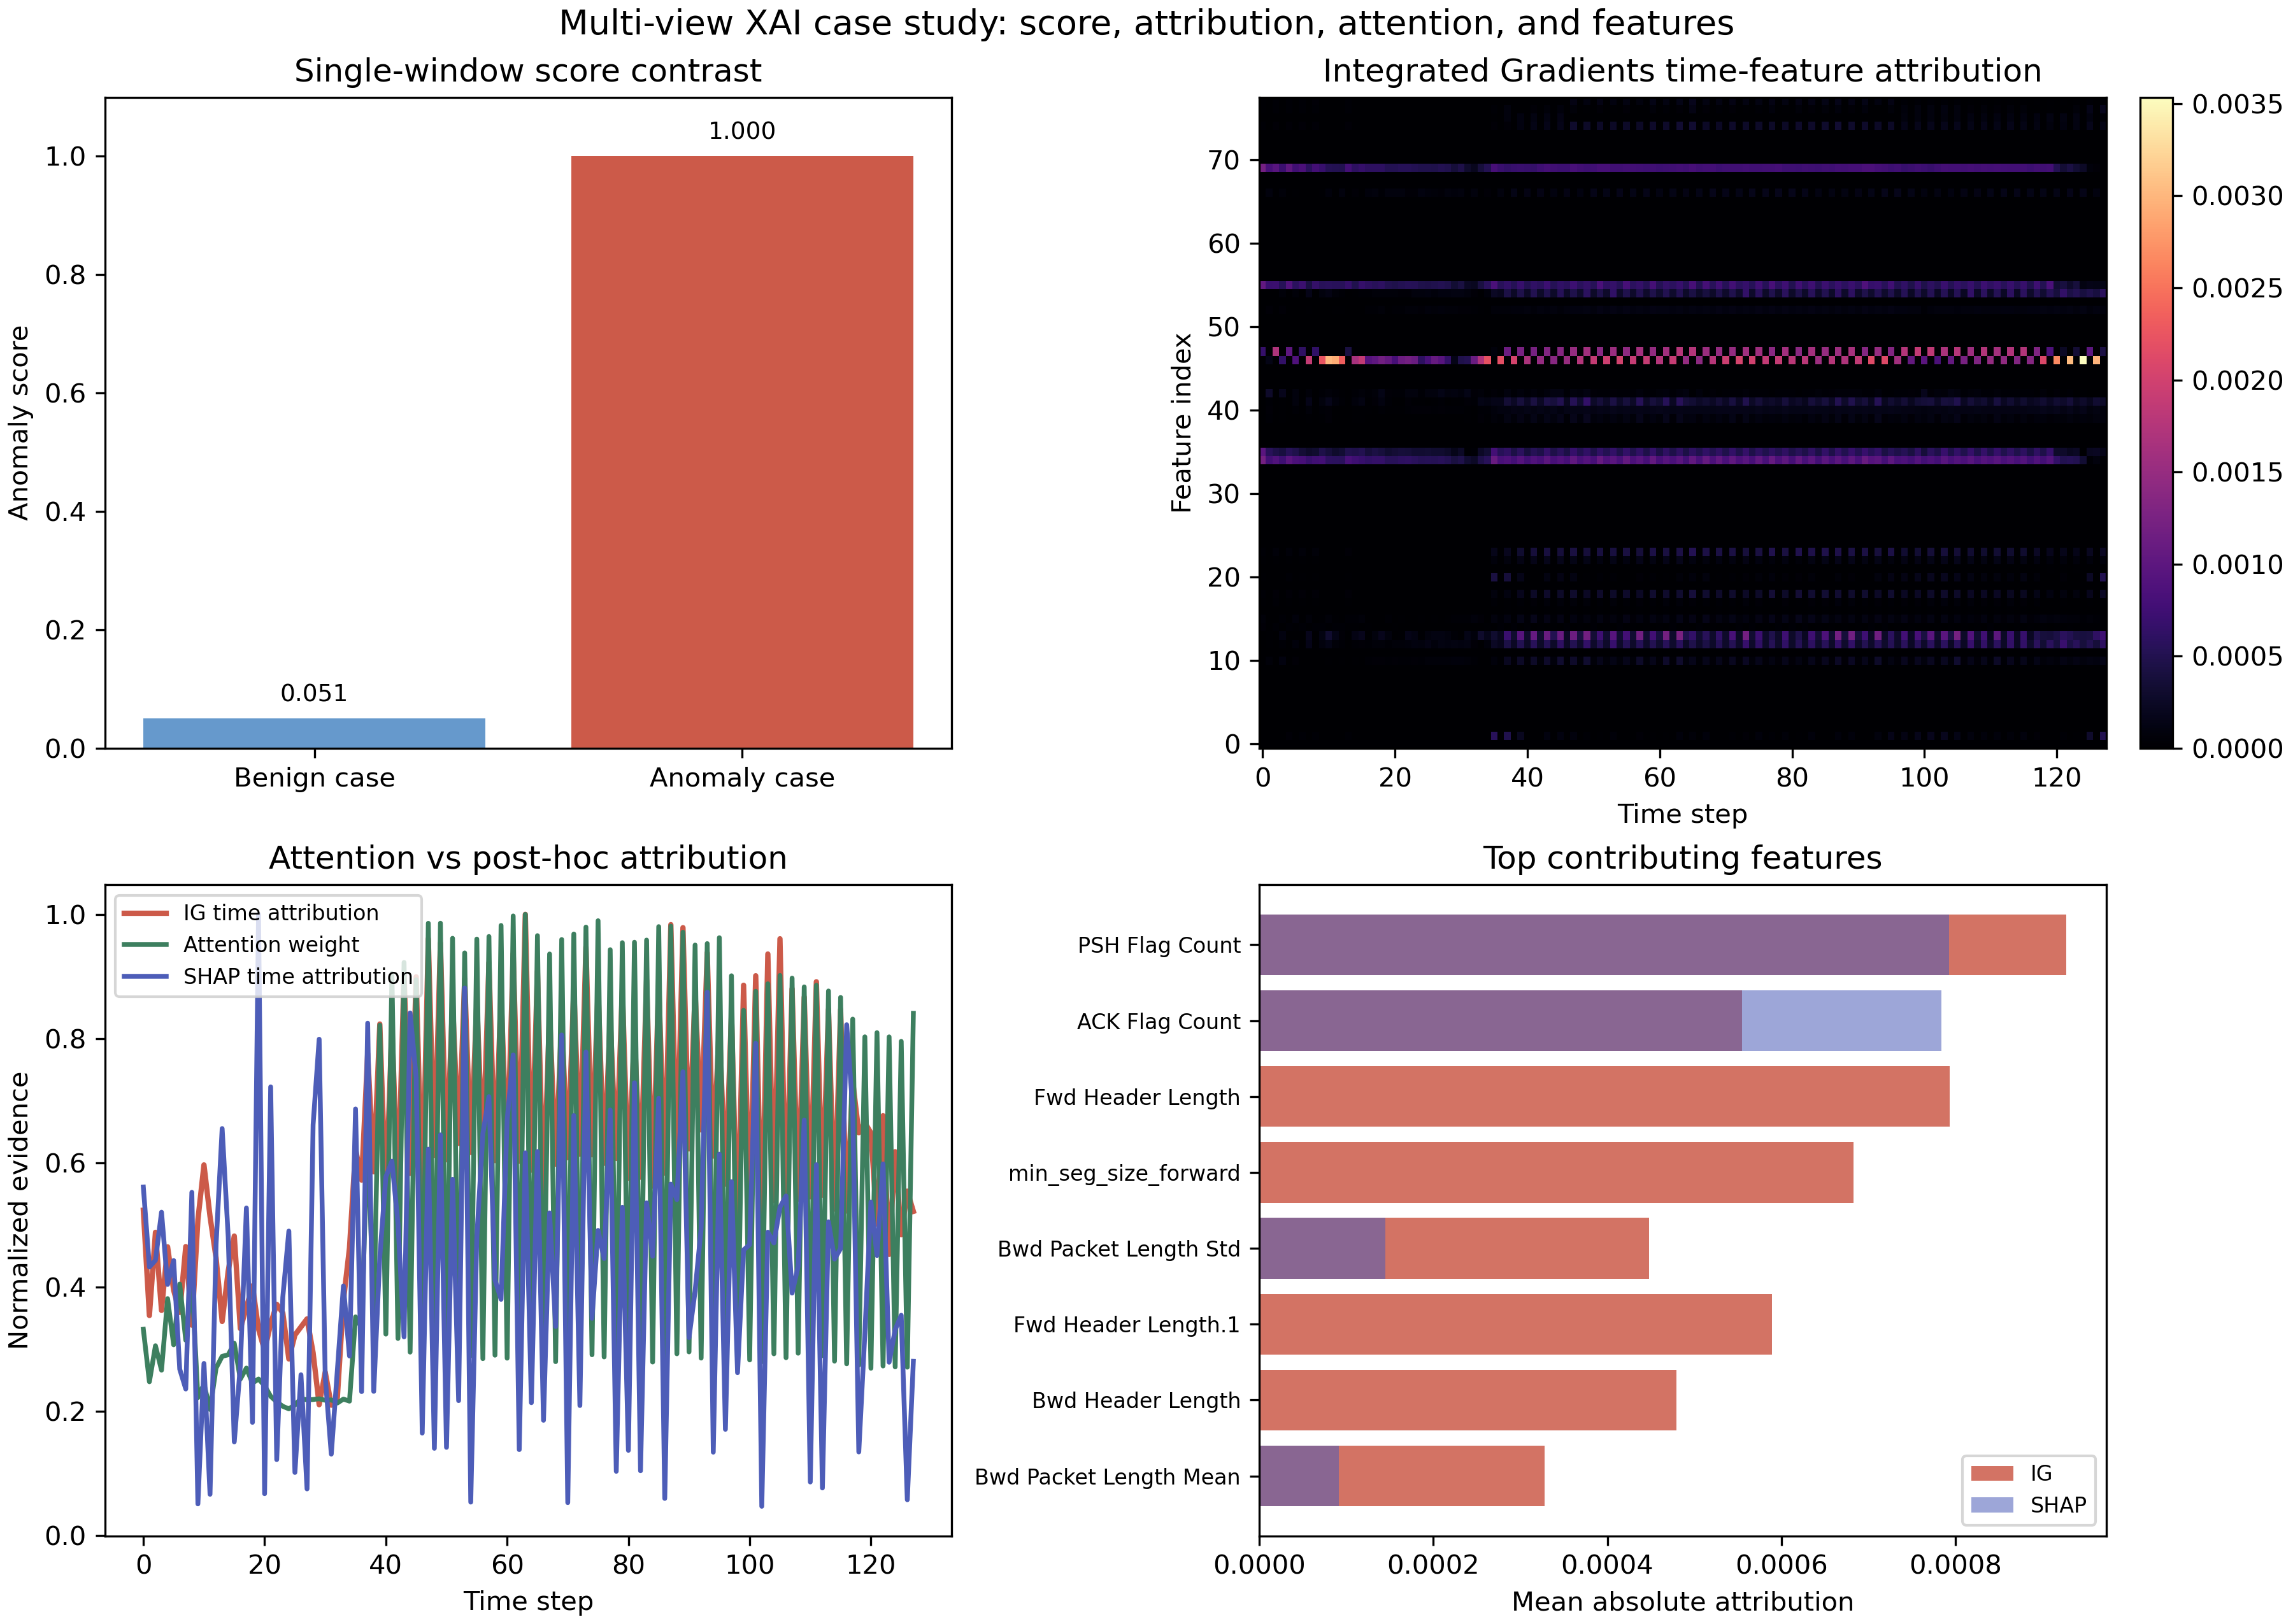
\includegraphics[width=\linewidth,height=0.36\textheight,keepaspectratio]{figures/xai_case_multiview_shap.png}
  \caption{Single-window multi-view XAI case study. The anomalous case has score 1.0000, while a benign reference case has score 0.0506. The figure compares attention, Integrated Gradients, SHAP, and top feature evidence.}
  \label{fig:xai-case}
\end{figure}

\begin{table}[!t]
  \centering
  \caption{Top-feature stability over 64 anomalous CICIDS2017 windows using gradient-times-input attribution. Coverage is the fraction of windows in which a feature appears in the window's top-5 attributed features.}
  \label{tab:xai-stability}
  \small
  \setlength{\tabcolsep}{3.2pt}
  \resizebox{\columnwidth}{!}{%
  \begin{tabular}{lccc}
    \toprule
    Feature & Top-5 Count & Coverage & Mean Rank \\
    \midrule
    PSH Flag Count & 53 & 0.828 & 1.23 \\
    Flow Packets/s & 42 & 0.656 & 2.74 \\
    Fwd Header Length.1 & 40 & 0.625 & 3.90 \\
    min\_seg\_size\_forward & 39 & 0.609 & 4.21 \\
    Destination Port & 33 & 0.516 & 3.45 \\
    \bottomrule
  \end{tabular}
  }
\end{table}

Fig.~\ref{fig:xai-case} shows a concrete alarm case with attention, Integrated Gradients, SHAP, and feature evidence. The most important features include TCP control flags, packet-rate statistics, header-length statistics, destination ports, and backward packet-length statistics. Table~\ref{tab:xai-stability} further shows that several feature groups recur across many anomalous windows rather than appearing only in one hand-picked example. The case study also illustrates why attention is not used alone: attention highlights temporal aggregation behavior, while Integrated Gradients and SHAP provide post-hoc evidence for the final anomaly score.

\section{Discussion}
The staged selection protocol is a pragmatic design choice. It makes the final comparison easier to interpret because the ablation changes only the model components under study, rather than changing window size, stride, and score fusion simultaneously.

The cross-dataset results refine the scope of the claim. CICIDS2017 is the primary benchmark on which the proposed detector is strongest, and SWaT provides a meaningful transfer check in an industrial-control setting. UNSW-NB15 should be interpreted as a stress test rather than as a second main win condition: the detector remains competitive, but the ranking among anomaly detectors changes under distribution shift and several methods trade substantially higher benign alarms for recall. TON\_IoT is more difficult still and is included as an explicit out-of-domain limitation. We therefore do not claim universal dominance across all network and telemetry domains. Instead, we claim that the proposed detector is particularly effective in the target low-FPR window-level IDS setting and that threshold transfer remains an important open problem.

For a deployable network security system, the most important lesson is that model accuracy and alarm policy should be evaluated together. Several baselines can obtain high recall only by increasing benign alarms, while strict calibration can reduce analyst burden but may miss attacks. The proposed framework makes this trade-off explicit by reporting both requested calibration budgets and observed test FPR. This also suggests a practical deployment path: calibrate thresholds on recent benign traffic from the target environment, monitor benign-alarm drift, and periodically refresh calibration rather than assuming that a fixed benchmark threshold will transfer unchanged.

The current XAI module should be interpreted as post-hoc analysis. It helps inspect whether model alarms are driven by stable temporal and feature-level evidence, but the current paper does not claim that the XAI signal improves training or provides a formal faithfulness guarantee. In particular, the paper does not claim that attention by itself is an explanation. A stronger future revision should add explicit faithfulness experiments, such as perturbing the highest-attention time steps and measuring score drops, before promoting attention auditability into a stand-alone methodological contribution.

The same caution applies to robustness and dataset coverage. The present paper includes only a lightweight Gaussian-noise check and does not yet include adversarial perturbation tests, explicit attack-type breakdown tables, or domain-adaptive training for TON\_IoT. We therefore treat those items as revision targets rather than as completed evidence.

\section{Ethical Considerations}
This work uses public benchmark network traffic data and does not run attacks against real systems. The primary risk is misuse or overclaiming: an intrusion detector trained on a benchmark may not generalize to all operational networks. We therefore report false positive rates, throughput, and limitations, and avoid presenting the model as a standalone replacement for human security operations. In deployment, the detector should be used as a triage aid whose alarms are reviewed together with logs, packet evidence, and existing security controls.

\section{Open Science and Artifact Availability}
The codebase contains scripts for staged tuning, baseline comparison, ablation, FPR-sweep analysis, seed runs, and XAI generation. For submission, the artifact should include anonymized source code, configuration files, plotting scripts, and instructions to reproduce the reported tables and figures.

\section{Conclusion}
This paper presents \model{} for low-false-positive, window-level network intrusion detection. The method combines temporal benign-window modeling, WGAN-GP training, and a Temporal Attention-Deviation (\tad{}) score that fuses attention-aware critic evidence with benign-reference feature deviation. On CICIDS2017, the final model outperforms same-granularity and modern anomaly-detection baselines at strict low-FPR operating points, and it transfers strongly to SWaT while remaining competitive on UNSW-NB15 under distribution shift. TON\_IoT marks the current boundary of cross-domain robustness rather than a claimed win. The ablation and XAI analyses further show that attention is most useful when paired with stable critic training and calibrated score fusion, and that alarms can be audited through complementary temporal and feature-level evidence. Overall, the results support a cautious but operationally relevant claim: low-noise NIDS alarms benefit from temporal benign-window modeling and calibrated score fusion, but deployment still requires environment-specific calibration and honest robustness boundaries.

\bibliographystyle{IEEEtran}
\bibliography{references}

\end{document}
